\documentclass[11pt,a4paper]{article}

\usepackage[margin=2.2cm]{geometry}
\usepackage[T1]{fontenc}
\usepackage[utf8]{inputenc}
\usepackage{lmodern}
\usepackage{microtype}
\usepackage{xcolor}
\usepackage{amsmath,amssymb,booktabs,enumitem,hyperref,graphicx,array}
\usepackage{fancyhdr}
\usepackage{titlesec}
\usepackage{tikz}
\usepackage{pgfplots}
\pgfplotsset{compat=1.18}

\definecolor{Ink}{HTML}{17212B}
\definecolor{Slate}{HTML}{34495E}
\definecolor{Sky}{HTML}{2D9CDB}
\definecolor{Mint}{HTML}{27AE60}
\definecolor{Sand}{HTML}{F4EDE4}
\definecolor{Paper}{HTML}{FBFCFD}
\definecolor{Accent}{HTML}{C0392B}

\pagecolor{Paper}
\color{Ink}

\hypersetup{
	colorlinks=true,
	linkcolor=Sky,
	urlcolor=Sky,
	citecolor=Sky,
	pdftitle={Part A Report},
	pdfauthor={Numerical Optimisation Project}
}

\pagestyle{fancy}
\fancyhf{}
\fancyhead[L]{\textcolor{Slate}{Numerical Optimisation Project}}
\fancyhead[R]{\textcolor{Slate}{Part A}}
\fancyfoot[C]{\textcolor{Slate}{\thepage}}
\setlength{\headheight}{24pt}
\renewcommand{\headrulewidth}{0.4pt}
\renewcommand{\headrule}{\hbox to\headwidth{\color{Sand}\leaders\hrule height \headrulewidth\hfill}}

\titleformat{\section}{\Large\bfseries\color{Ink}}{}{0pt}{}
\titleformat{\subsection}{\large\bfseries\color{Slate}}{}{0pt}{}
\titleformat{\subsubsection}{\bfseries\color{Ink}}{}{0pt}{}

\setlist[itemize]{leftmargin=1.4em,itemsep=0.35em,topsep=0.35em}
\setlength{\parskip}{0.55em}
\setlength{\parindent}{0pt}

\newcommand{\resultcard}[2]{%
\begin{tikzpicture}
	\node[rounded corners=10pt, fill=white, draw=Sand, line width=0.8pt, inner sep=10pt, minimum width=0.3\linewidth] (box) {\begin{minipage}{0.85\linewidth}\centering\textcolor{Slate}{#1}\\[0.35em]{\Large\bfseries #2}\end{minipage}};
\end{tikzpicture}}

\begin{document}

\hypersetup{pageanchor=false}
\begin{titlepage}
\thispagestyle{empty}
\begin{tikzpicture}[remember picture,overlay]
	\fill[Ink] (current page.north west) rectangle ([yshift=-4.5cm]current page.north east);
	\fill[Sky] ([yshift=-4.5cm]current page.north west) rectangle ([yshift=-4.8cm]current page.north east);
	\fill[Sand] ([yshift=-18.4cm]current page.north west) rectangle (current page.south east);
\end{tikzpicture}

\vspace*{2.1cm}
{\color{white}\huge\bfseries Numerical Optimisation Project\par}
\vspace{0.55cm}
{\color{white}\LARGE Part A: Farm Planning Model\par}
\vspace{1.3cm}

\begin{minipage}{0.92\textwidth}
\color{white}
This report presents the Part A farm-planning model: a JuMP/Gurobi optimisation that allocates crops, pumping, hired labour, and sales to maximize gross margin under land, water, labour, and market constraints.
\end{minipage}

\vfill
\begin{minipage}{0.92\textwidth}
\color{white}
\textbf{Focus of this report}\par
\smallskip
Clear formulation, clean implementation blocks, and result graphs that can be discussed quickly during an oral exam.
\end{minipage}

\vspace*{1.7cm}
\end{titlepage}

\clearpage
\hypersetup{pageanchor=true}
\pagenumbering{arabic}
\setcounter{page}{1}

\tableofcontents
\newpage

\section{Part A: Farm Planning Model}

\subsection{Executive Summary}

Part A solves a crop planning problem with irrigation and labour decisions. The model chooses the crop mix, pumping, hiring, and sales strategy that maximizes annual gross margin under the farm constraints.

\begin{center}
\small
\renewcommand{\arraystretch}{1.18}
\begin{tabular}{>{\raggedright\arraybackslash}p{0.22\textwidth} >{\centering\arraybackslash}p{0.18\textwidth} >{\centering\arraybackslash}p{0.22\textwidth} >{\centering\arraybackslash}p{0.18\textwidth}}
\toprule
\textbf{Objective value} & \textbf{Pump licence} & \textbf{Final reservoir} & \textbf{Peak labour} \\
\midrule
\$122{,}077.77 & 100\% & 10{,}000 m$^3$ & 125 h \\
\bottomrule
\end{tabular}
\end{center}

\subsection{Model in One View}

The problem uses three sets: land blocks $B$, crops $C$, and periods $T$. The model selects area variables $x_{b,c}$, pumping $p_t$, reservoir level $r_t$, hired labour $h_t$, and sales variables for each crop.

\begin{itemize}[leftmargin=1.5em]
    \item Objective: maximize revenue minus crop cost, hired labour cost, and pumping cost.
    \item Key trade-off: more irrigation and labour allow higher-value crops, but each resource is capped.
    \item Structure: the code is split into clear blocks in \texttt{src/model.jl} so each component can be modified independently.
\end{itemize}

\subsection{Input Data}

The implementation reads the following CSV files:

\begin{itemize}[leftmargin=1.5em]
    \item \texttt{blocks.csv}: land blocks, area, and soil class.
    \item \texttt{crops.csv}: crop parameters such as variable costs and farm share limits.
    \item \texttt{yields.csv}: yield by crop and soil class.
    \item \texttt{calendar.csv}: irrigation and labour requirements by period.
    \item \texttt{labour.csv}: family labour, hired labour capacity, and hired labour cost.
    \item \texttt{water.csv}: inflows and pumping limits.
    \item \texttt{markets.csv}: prices and contract information.
    \item \texttt{parameters.csv}: global constants such as reservoir capacity and pumping cost.
\end{itemize}

These inputs are loaded into a single \texttt{FarmData} structure in \texttt{src/data.jl}.

\subsection{Decision Variables}

\begin{align*}
    x_{b,c} &\ge 0 && \text{area of crop } c \text{ on block } b, \\
    p_t &\ge 0 && \text{water pumped in period } t, \\
    r_t &\ge 0 && \text{reservoir level at the end of period } t, \\
    s_t &\ge 0 && \text{spill in period } t, \\
    h_t &\ge 0 && \text{hired labour in period } t, \\
    q^{\text{contract}}_c &\ge 0 && \text{contracted sales of crop } c, \\
    q^{\text{spot}}_c &\ge 0 && \text{spot sales of crop } c.
\end{align*}

\subsection{Model Logic}

\paragraph{Land allocation}
Each block is fully assigned across crops, and each crop has a maximum farm share.

\paragraph{Production and sales}
Production is computed from area and yield. It is then split into contract and spot sales when a market exists.

\paragraph{Water system}
The reservoir evolves period by period using inflow, pumping, irrigation use, and spill. Reservoir capacity and annual pumping licence both bind the water system.

\paragraph{Labour system}
Family labour and hired labour together cover crop labour needs, while hired labour itself is capped each period.

\subsection{Graphs and Results}

\begin{figure}[htbp]
\centering
\begin{tikzpicture}
\begin{axis}[
    ybar stacked,
    bar width=10pt,
    width=0.95\textwidth,
    height=7cm,
    ymin=0,
    ylabel={Area (ha)},
    xlabel={Block},
    symbolic x coords={B1,B2,B3,B4},
    xtick=data,
    nodes near coords,
    nodes near coords align={vertical},
    every axis plot/.append style={fill opacity=0.92},
    legend style={at={(0.5,1.08)},anchor=south,legend columns=3,draw=none,fill=none},
    enlarge x limits=0.12,
    axis line style={draw=Slate},
    tick style={draw=Slate},
    title={Optimal crop allocation by block}
]
\addplot+[fill=Sky] coordinates {(B1,0) (B2,18.0) (B3,0) (B4,14.0)};
\addplot+[fill=Mint] coordinates {(B1,0) (B2,0.848678) (B3,11.29648) (B4,0)};
\addplot+[fill=Accent] coordinates {(B1,11.106383) (B2,3.151322) (B3,0) (B4,0)};
\addplot+[fill=Slate] coordinates {(B1,14.893617) (B2,0) (B3,0) (B4,0)};
\addplot+[fill=Sand] coordinates {(B1,0) (B2,0) (B3,3.2) (B4,0)};
\legend{Winter wheat, Winter barley, Sugar beet, Potato, Cover fallow}
\end{axis}
\end{tikzpicture}
\caption{The optimal crop mix concentrates value in sugar beet and potato on block B1, uses winter cereals on B2 and B4, and leaves a cover-fallow area on B3.}
\end{figure}

\begin{figure}[htbp]
\centering
\begin{tikzpicture}
\begin{axis}[
    width=0.9\textwidth,
    height=6.2cm,
    ymin=0,
    ylabel={m$^3$},
    xlabel={Period},
    symbolic x coords={P1,P2,P3,P4},
    xtick=data,
    nodes near coords,
    every axis plot/.append style={fill=Sky},
    axis line style={draw=Slate},
    tick style={draw=Slate},
    title={Pumping profile}
]
\addplot+[ybar] coordinates {(P1,0) (P2,4000) (P3,5000) (P4,1000)};
\end{axis}
\end{tikzpicture}
\caption{Water use is concentrated in P2--P4, and the annual pumping licence is fully used.}
\end{figure}

\begin{figure}[htbp]
\centering
\begin{tikzpicture}
\begin{axis}[
    width=0.9\textwidth,
    height=6.2cm,
    ymin=0,
    ylabel={Hours},
    xlabel={Period},
    symbolic x coords={P1,P2,P3,P4},
    xtick=data,
    nodes near coords,
    every axis plot/.append style={fill=Mint},
    axis line style={draw=Slate},
    tick style={draw=Slate},
    title={Hired labour profile}
]
\addplot+[ybar] coordinates {(P1,0) (P2,0) (P3,0) (P4,125)};
\end{axis}
\end{tikzpicture}
\caption{Hired labour is only required in the final period, where the labour cap binds.}
\end{figure}

\begin{table}[htbp]
\centering
\caption{Selected solution values from the optimal Part A run}
\begin{tabular}{lrrrr}
\toprule
\textbf{Crop} & \textbf{Contracted sales} & \textbf{Spot sales} & \textbf{Total} & \textbf{Comment} \\
\midrule
Winter wheat & 302.40 & 0.00 & 302.40 & Contracted \\
Winter barley & 98.72 & 0.00 & 98.72 & Contracted \\
Grain maize & 42.04 & 0.00 & 42.04 & Contracted \\
Sugar beet & 1199.30 & 0.00 & 1199.30 & Contracted \\
Potato & 700.00 & 0.00 & 700.00 & Contracted \\
Field beans & 0.00 & 0.00 & 0.00 & Not used \\
\bottomrule
\end{tabular}
\end{table}

\subsection{Implementation Notes}

The code is organized in \texttt{src/model.jl} into separate blocks for data preparation, land constraints, market constraints, resource constraints, and the objective function.

That structure is intentionally kept simple so it can be explained and modified quickly during an oral exam.

\subsection{Interpretation}

The optimal plan uses the available water licence fully, hits the reservoir terminal target, and requires hired labour only in the last period. The crop pattern shows the model balancing high-margin crops against water and labour scarcity.

\subsection{Current Scope}

This report intentionally covers only Part A for now. The document and codebase can be extended later with sensitivity analysis, Part B/C formulations, or comparison against alternative crop plans.

\end{document}